
\chapter{ESTIMATORS}
\label{chap:Estimators}

Section \ref{chap:StateError} explained the rationale for the state representations and how adjustments can be applied to them in a manner than preserves the integrity of it's connection to the TableSat/MMS's physical orientation.  Usage of the gains are also done to make the effects of gain tuning more intuitive.

\section{State Prediction}
\label{sec:StatePrediction}

Section \ref{sec:BodyRatePIDEstimation} shows that to keep accurate tracking of a spin-stabilized satellite like TableSat or MMS, the system's dynamic equations are required to couple the body rate and quaternion values.  This is especially important for the TableSat 1A implementation since only the magnetometer and course sun sensors provide feedback about the system's state, and they only have a partial measurement of the attitude quaternion and no direct measurement of the body rates.

The approach taken in the TSatPy code to create state predictions off previous state estimates is to start with a discretized Euler's Moment Equations \ref{eqn:DiscreteEulerMomentEquations} to predict $\bs{\dot{\omega}}(t_{k+1})$.  The the current estimated body rate is adjusted based on the variable time step size.

\begin{equation}
  \bs{\omega}(t_{k+1}) = \bs{\omega}(t_{k}) + \bs{\dot{\omega}}(t_{k+1})\cdot (t_{k+1} - t_k)
\end{equation}

The newly estimated body rates $\bs{\omega}(t_{k+1})$ are supplied to the discretized quaternion dynamics Equation \ref{eqn:DiscreteQuaternionPropagation} to calculate the newly estimated rotational quaternion.

\section{PID State Estimation}
\label{sec:BodyRatePIDEstimation}

This section will cover the use of PID adjustments to track state estimation.  Section \ref{chap:StateError} covered how states and especially the quaternion portion can be scaled.  The same method can be applied to the proportional part of the PID estimator.

\subsection{Proportional State Estimation}
\label{subsec:ProportionalEstimator}

The proportional estimator defined in Equation \ref{eqn:PEstimator} was implemented in TSatPy.  Taking the estimated and measured states from Equation \ref{eqn:StateDifferenceQuaternionSamples}, an update of the TableSat/MMS state estimate is performed in the following manner.

\begin{subequations}
  \begin{align}
    \bs{\hat{x}}(t_{k+1}) &= \begin{bmatrix} \bs{\hat{q}}(t_{k+1}) \\ \bs{\hat{\omega}}(t_{k+1}) \end{bmatrix} \\
    \bs{\hat{q}}(t_{k+1}) &= \bs{\psi}(\bs{q}_e(t_{k}), K_{qp}) \otimes \bs{\hat{q}}(t_{k}) \\
    \bs{\hat{\omega}}(t_{k+1}) &= \bs{\hat{\omega}}(t_{k}) + \bs{K}_{\omega p} \cdot \bs{\omega}_e(t_{k})
  \end{align}
  \label{eqn:PEstimator}
\end{subequations}

\begin{singlespace}
  \begin{minted}[mathescape,linenos,numbersep=10pt,frame=lines,framesep=2mm]{python}
from TSatPy import StateOperator, Estimator, State
from TSatPy.Clock import Metronome
import numpy as np

x_ic = State.State(
    State.Quaternion([0,0,1],radians=190/180.0*np.pi),
    State.BodyRate([0,0,3]))
print("x_ic:    %s" % (x_ic))

k = 0.2
Kp = StateOperator.StateGain(
    StateOperator.QuaternionGain(k),
    StateOperator.BodyRateGain(np.eye(3) * k))
print("Kp:  %s" % (Kp))

c = Metronome()
pid = Estimator.PID(c, ic=x_ic)
pid.set_Kp(Kp)
print("pid: %s" % (pid))

x_m = State.State(
    State.Quaternion([0,0.1,1],radians=44/180.0*np.pi),
    State.BodyRate([0,0,3.1]))
pid.update(x_m)
print("pid.x_hat:   %s" % (pid.x_hat))

e, r = pid.x_hat.q.to_rotation()
print("e:      <%g, %g, %g>\ndegree: %g" % (
    e[0,0],e[1,0],e[2,0], r * 180.0 / np.pi))

# Prints Out
# x_ic:    <Quaternion [-0 -0 -0.996195], -0.0871557>,
#          <BodyRate [0 0 3]>
# Kp:  <StateGain <Kq 0.2>,
#      <Kw = [[ 0.2 0. 0. ] [ 0. 0.2 0. ] [ 0. 0. 0.2]]>>
# pid: PID
#  x_hat <Quaternion [-0 -0 -0.996195], -0.0871557>, <BodyRate [0 0 3]>
#  Ki None
#  Kp <StateGain <Kq 0.2>,
#     <Kw = [[ 0.2 0. 0. ] [ 0. 0.2 0. ] [ 0. 0. 0.2]]>>
#  Kd None
# pid.x_hat:   <Quaternion [-0.00170765 0.00968454 -0.985915], 0.16696>,
#              <BodyRate [0 0 3.02]>
# e:      <-0.00173196, 0.00982241, -0.99995>
# degree: 160.778
  \end{minted}
\nocite{minted}
\end{singlespace}

This demonstrates that a proportional estimator initialized to a state of a $190^o$ rotation about $+z$-axis and a body rate of $\omega_z = 3$ rad/sec.  The proportional gain applied to state errors is set to $0.2$ for the quaternion and all body rates.  After the measured state of a $44^o$ rotation about the axis $0 \bs{i} + 0.1 \bs{j} + 1\bs{k}$ and a body rate of $\omega_z = 3.1$ rad/sec is applied, the new estimated state is a $160.778^o$ degree rotation about $0.00173196 \bs{i} - 0.00982241 \bs{j} + 0.99995\bs{k}$ with a body rate of $3.02$ rad/sec.

\begin{figure}[H]
  \centerline{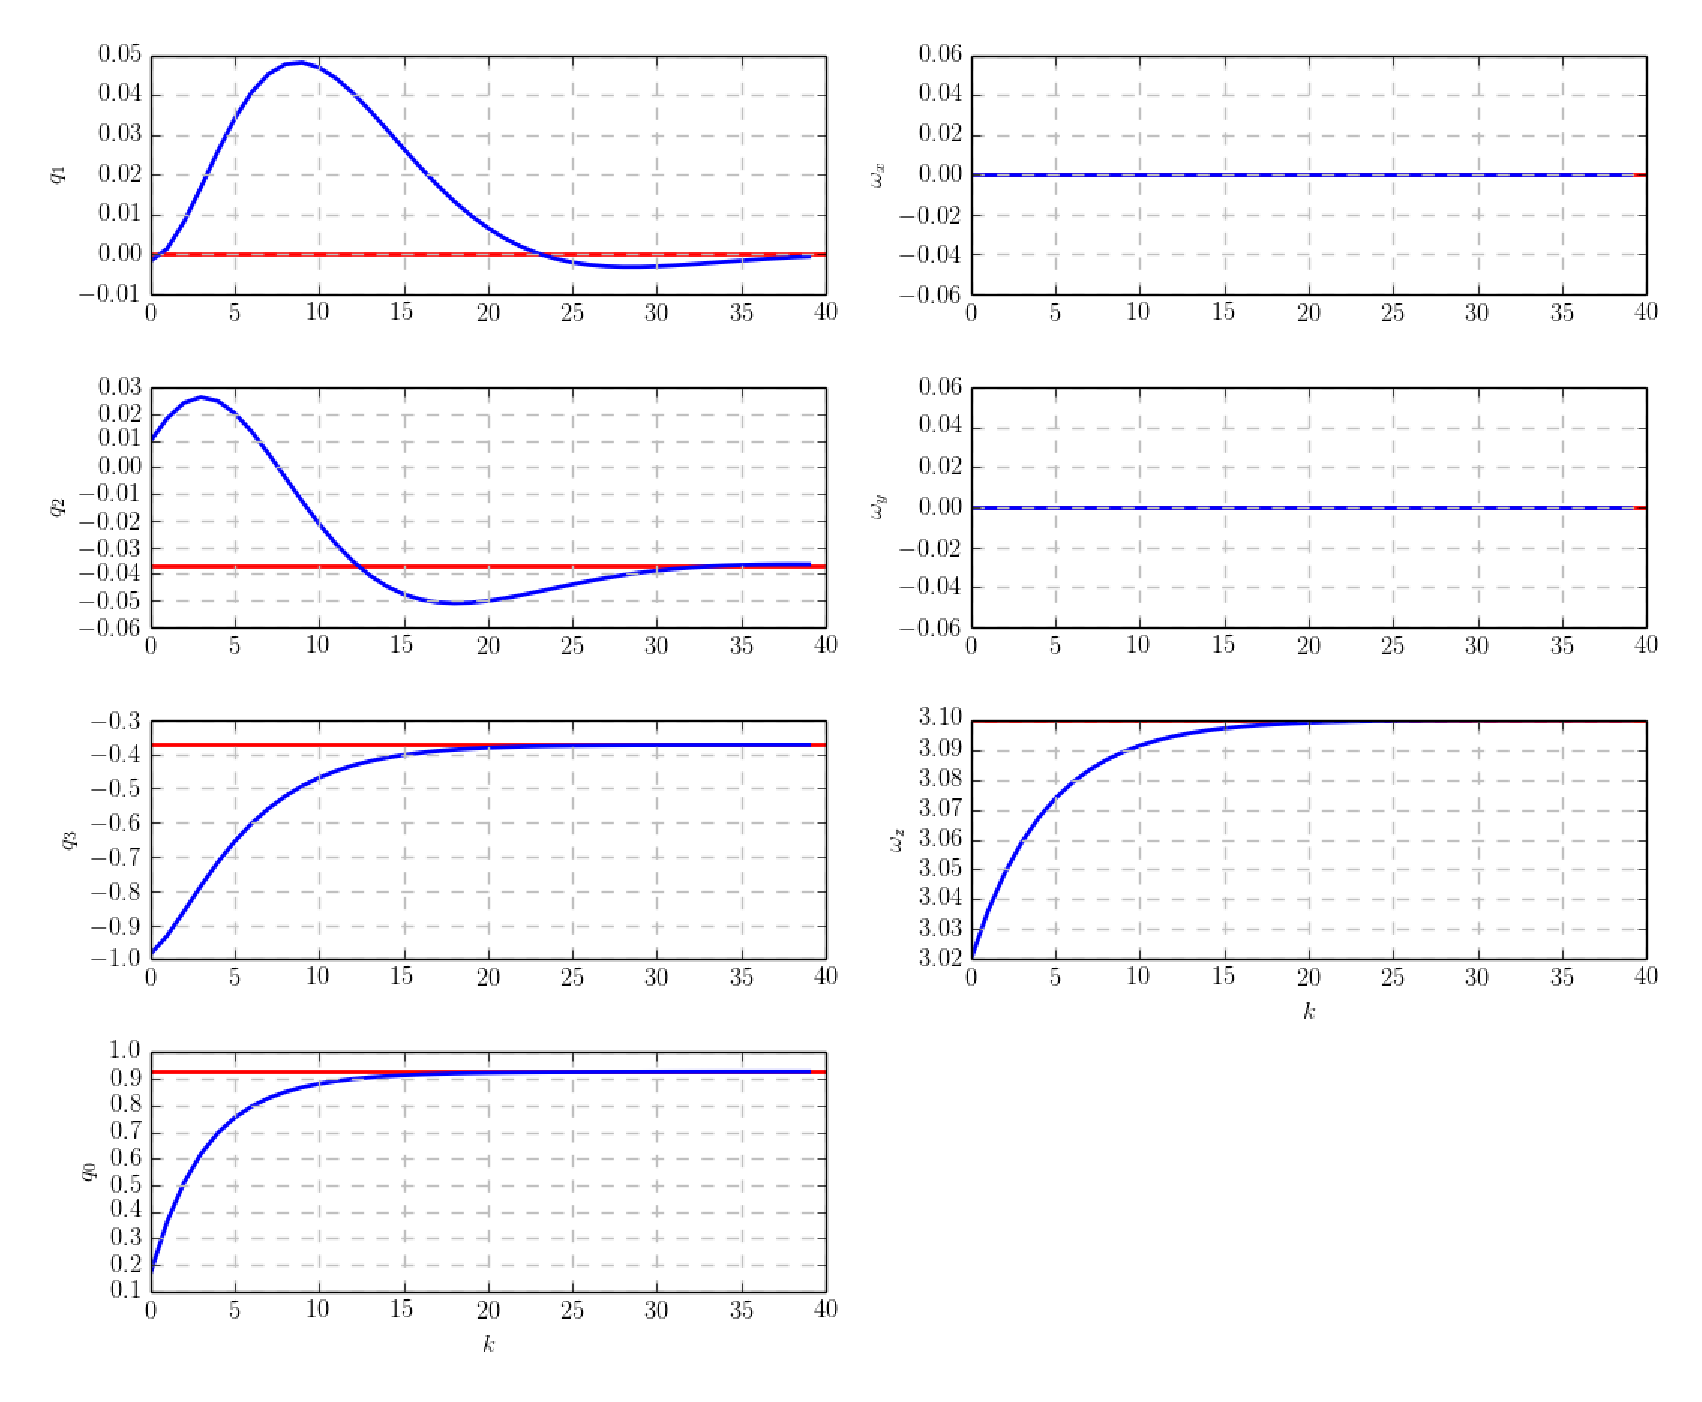
\psfig{file=figures/p_estimator_static_target.eps,width=6in}}
  \caption{P-Estimator with static target}
  \label{fig:PEstimatorwithstatictarget}
\end{figure}

The work covered so far in this chapter has all dealt with the a system in a static state.  In Figure \ref{fig:PEstimatorwithstatictarget}, a P-Estimator converges it's estimated state (blue) to the static measured state (red).  While the estimated state converges to the measured state after about 40 iterations, this type of conversion would be effective only for non-rotating systems.  The non-zero $\omega_z$ means that the quaternion attitude representation will be in constant motion.

The $3.1$ rad/sec rotation about $0\bs{i} + 0.1\bs{j} + 1\bs{k}$ condition from the previous p-estimator is then allowed to propagate the quaternion state through 10 second of rotation with state estimate updates every 0.1 sec.  The resulting measured state (red) and estimated state (blue) is shown in Figure \ref{fig:PEstimatorwithrotatingtarget}.  The body rates track identically to those in Figure \ref{fig:PEstimatorwithstatictarget} where $t(k) = 2$ corresponds to $k = 20$.  Due to the proportional only compensation and no predictive methods, the initial transient behavior is followed by a behavior similar to a steady state error.

\begin{figure}[H]
  \centerline{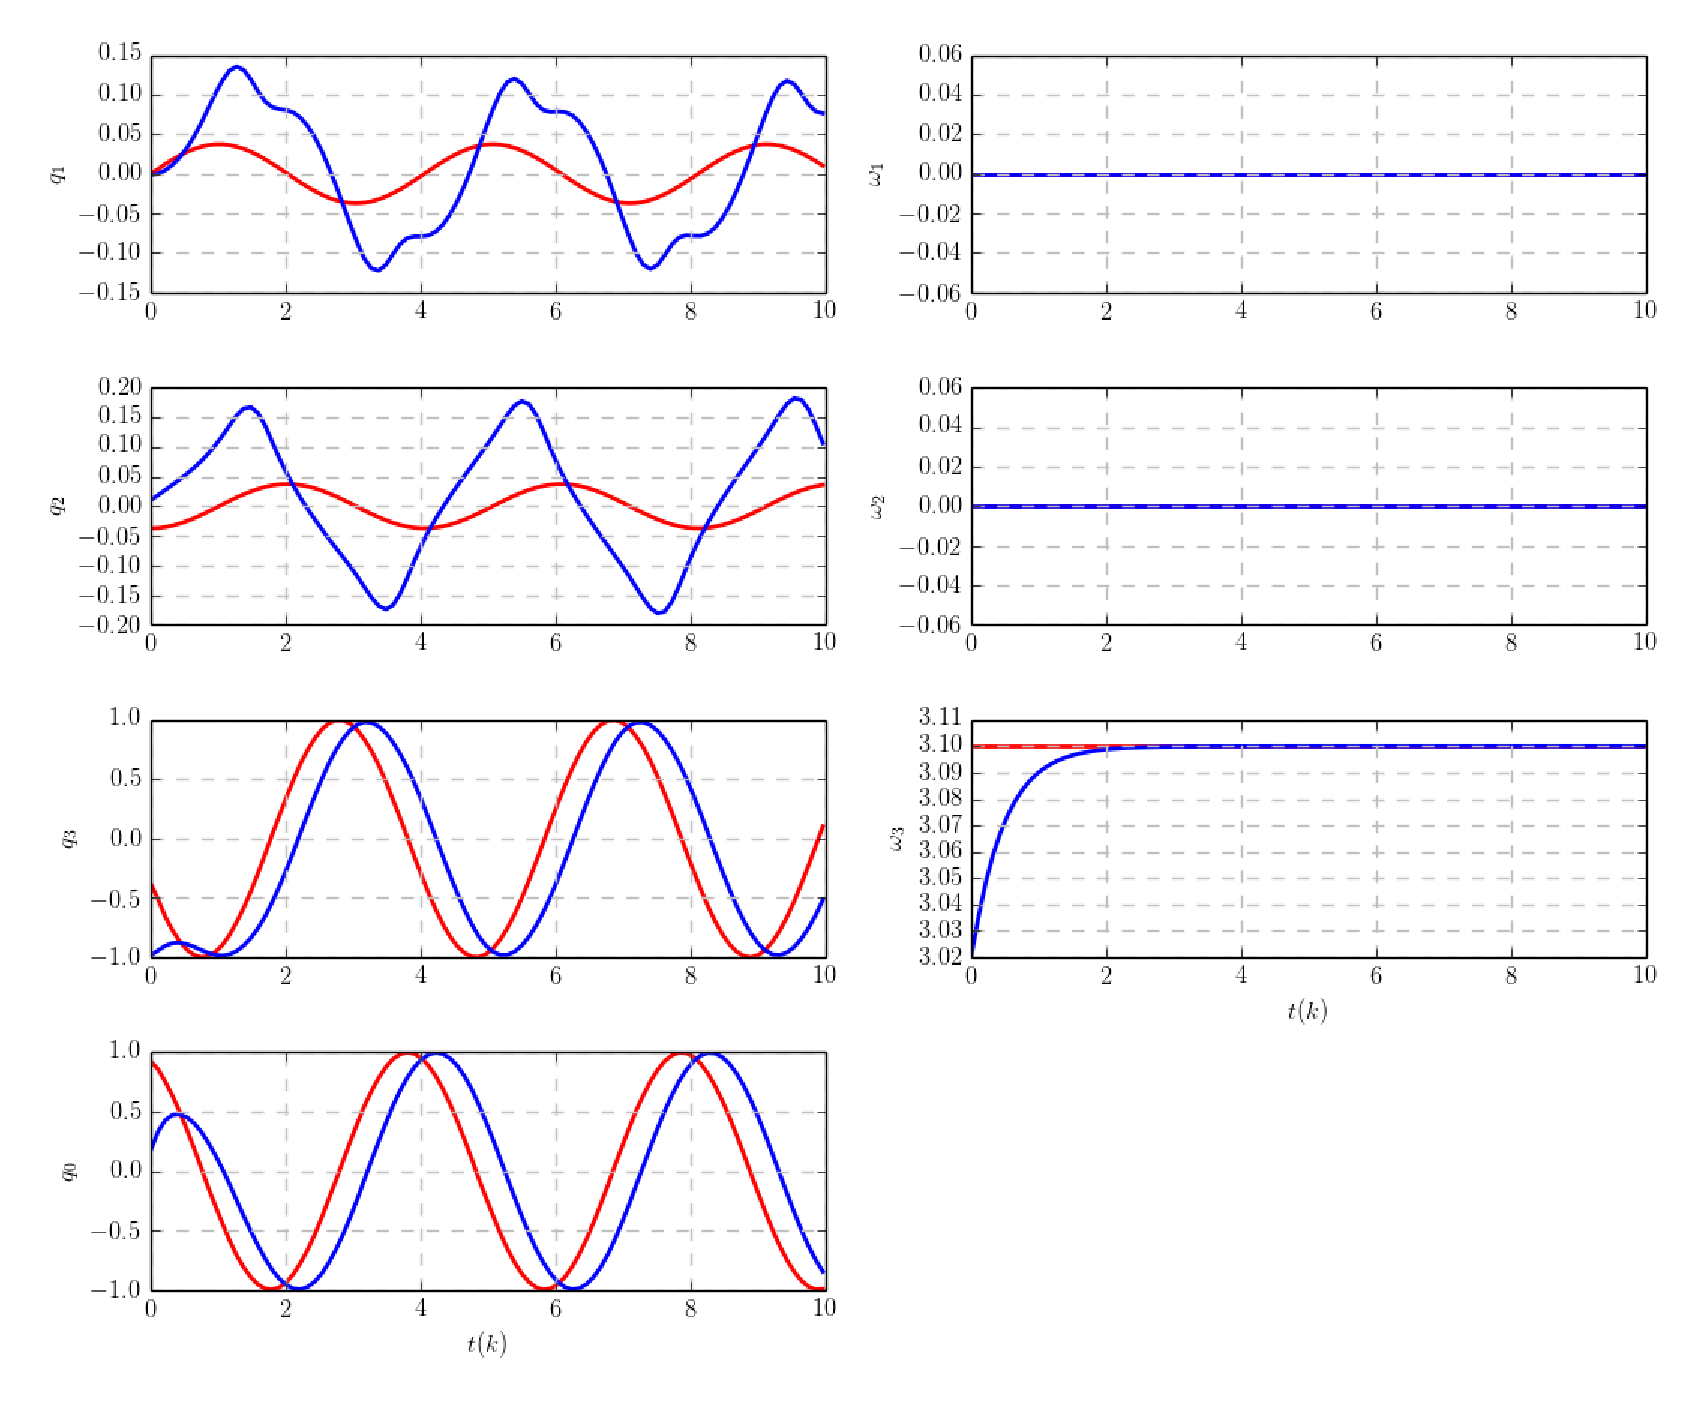
\psfig{file=figures/p_estimator_3radps.eps,width=6in}}
  \caption{P-Estimator with rotating target}
  \label{fig:PEstimatorwithrotatingtarget}
\end{figure}

Increasing the frequency of updates to the p-estimator can decrease the error between the measured and estimated states, but there will always be an error similar to a steady state error in the quaternion representation.  For better results the estimator needs to take into consideration changes in the state through the PID's integration and derivative terms.

\subsection{Integral State Estimation}
\label{subsec:IntegralEstimator}

To stay consistent with the findings in State Error (Chapter \ref{chap:StateError}), the quaternion portion of the integrated state should abide by the quaternion multiplicative correction method.  This is the first model where the variable sized time step is also taken into consideration.  Instead of accumulating the error measurements, the error corrections should be weighted according to the length of time between updates $t(k+1) - t(k)$.  In a simplified case the integral term should end up the same in the following two update instances.

\begin{table}[H]
  \centering
  \begin{tabular}{r|c|c|c|c|c}
    $t_1 (sec)$ & 0.1 & 0.2 & 0.3 & 0.4 & 0.5 \\ \hline
    $\theta_e$ & 4 & -3 & -3 & -3 & 5 \\
    \\
    $t_2 (sec)$ & 0.1 & & & 0.4 & 0.5 \\ \hline
    $\theta_e$ & 4 &  &  & -3 & 5 \\
  \end{tabular}
  \label{tbl:VariableUpdates}
\end{table}

In $t_1$, regular updates occur every 0.1 sec ending in an integral error value of 0.  In $t_2$, without taking into consideration the variable step sizes would end in an error value of $+6$, but really the -3 error update should be worth three times as much.

Running the state estimator without compensating for variations in time step sizes can create inconsistencies between different experimental runs.  In Figure \ref{fig:IEstimatorwithouttimevariationcompensation}, the integral estimator was updated with a fixed state for 30 seconds.  The estimator was initialized at $0$ radians and run three times against a fixed angle of $0.5$ radians.  The first time with an estimation update frequency of every 0.4 seconds (blue), second with the update frequency of every 0.1 seconds (red), and third with a variable update frequency (green) that jumped back and forth between updating every 0.05 and 0.4 seconds.

\begin{figure}[H]
  \centerline{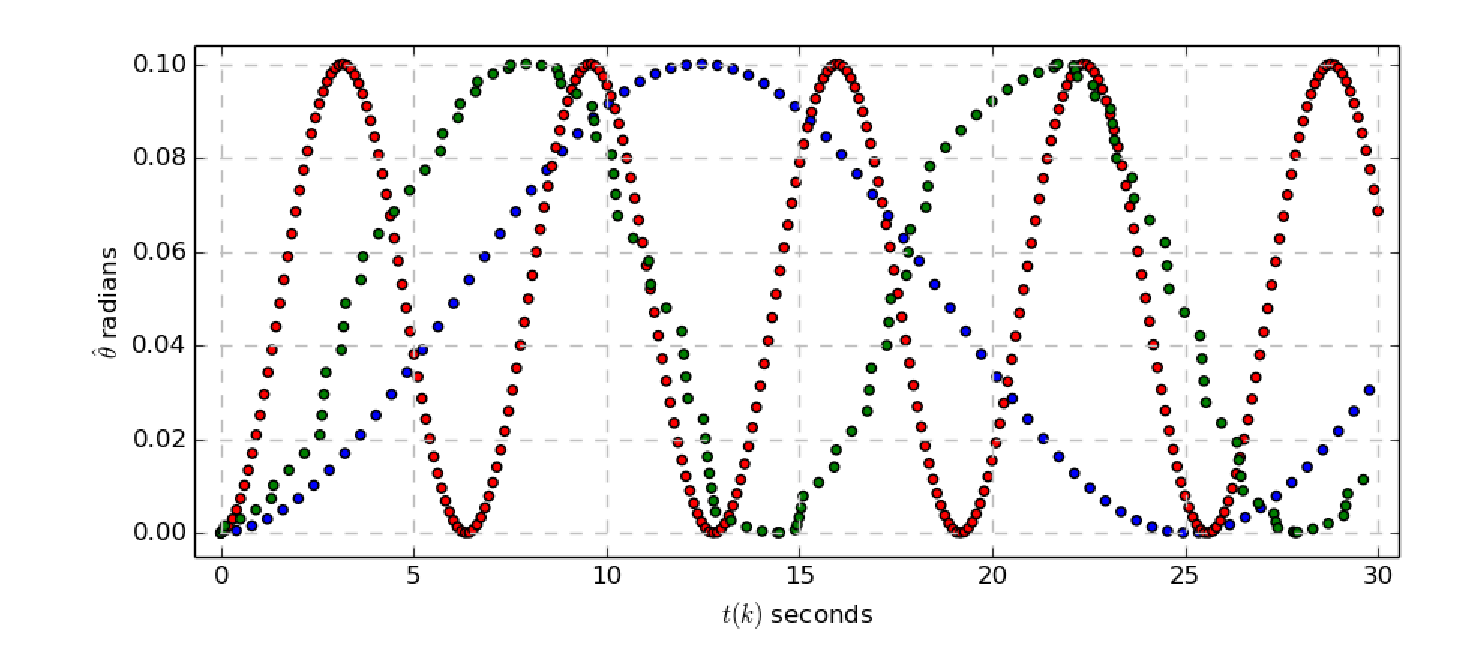
\psfig{file=figures/i_estimator_no_time_varying.eps,width=6in}}
  \caption{I-Estimator without time variation compensation}
  \label{fig:IEstimatorwithouttimevariationcompensation}
\end{figure}

Each calculated estimate for $\hat{\theta}$ in the $k$ domain is identical for each of the three runs, but varies greatly in the time domain.  Most notably, the third run that alternates between update frequencies ends up creating an estimation dynamic that could make the controller less robust.

In comparison, the PID estimator was modified to incorporate the time step size into it's integral term.  The same three tests were run as above with the 0.1 (red), 0.4 (blue), and variable 0.05/0.4 (green) time steps.  The adjustment quaternion method from Section \ref{sec:HighIntegrityStateAdjustments} is first used to compensate for measured time step size of $\Delta t_{k}$ creating a consistent error quaternion. then is used as before to scale the error quaternion by the selected gain value.  The results of this work can be seen in Figure \ref{fig:IEstimatorwithtimevariationcompensation} where the three test runs are still not identical, but their dynamics are more similar than before.  More notably, the variable step test (green) shows less variability in the estimate being produced which will reduce the noise being transferred to the control algorithm.

\begin{subequations}
  \begin{align}
    \bs{\hat{x}}(t_{k+1}) &= \begin{bmatrix} \bs{\hat{q}}(t_{k+1}) \\ \bs{\hat{\omega}}(t_{k+1}) \end{bmatrix} \\
    \bs{\hat{q}}(t_{k+1}) &= \bs{\psi}\big(\bs{q}_{ei}(t_k), K_{qi}\big) \otimes \bs{\hat{q}}(t_{k}) \\
    \bs{q}_{ei}(t_k) &= \bs{\psi}(\bs{q}_e(t_{k}), \Delta t_{k}) \otimes \bs{q}_{ei}(t_{k-1})\\
    \bs{\hat{\omega}}(t_{k+1}) &= \bs{\hat{\omega}}(t_{k}) + \bs{K}_{\omega i} \cdot (\Delta t_k \bs{I})\cdot \bs{\omega}_e(t_{k})
  \end{align}
  \label{eqn:IEstimator}
\end{subequations}

In Equation \ref{eqn:IEstimator}, the error quaternion $\bs{q}_{ei}(t_k)$ used is an accumulation of the time step scaled errors encountered in all previous steps.  This is analogous to a running summation of the error values.  For the body rate estimation, it's largely the traditional integral component with an extra $\Delta t_k \bs{I}$ term that linearly scales the body rate error calculations based on the size of the current time step.

\begin{figure}[H]
  \centerline{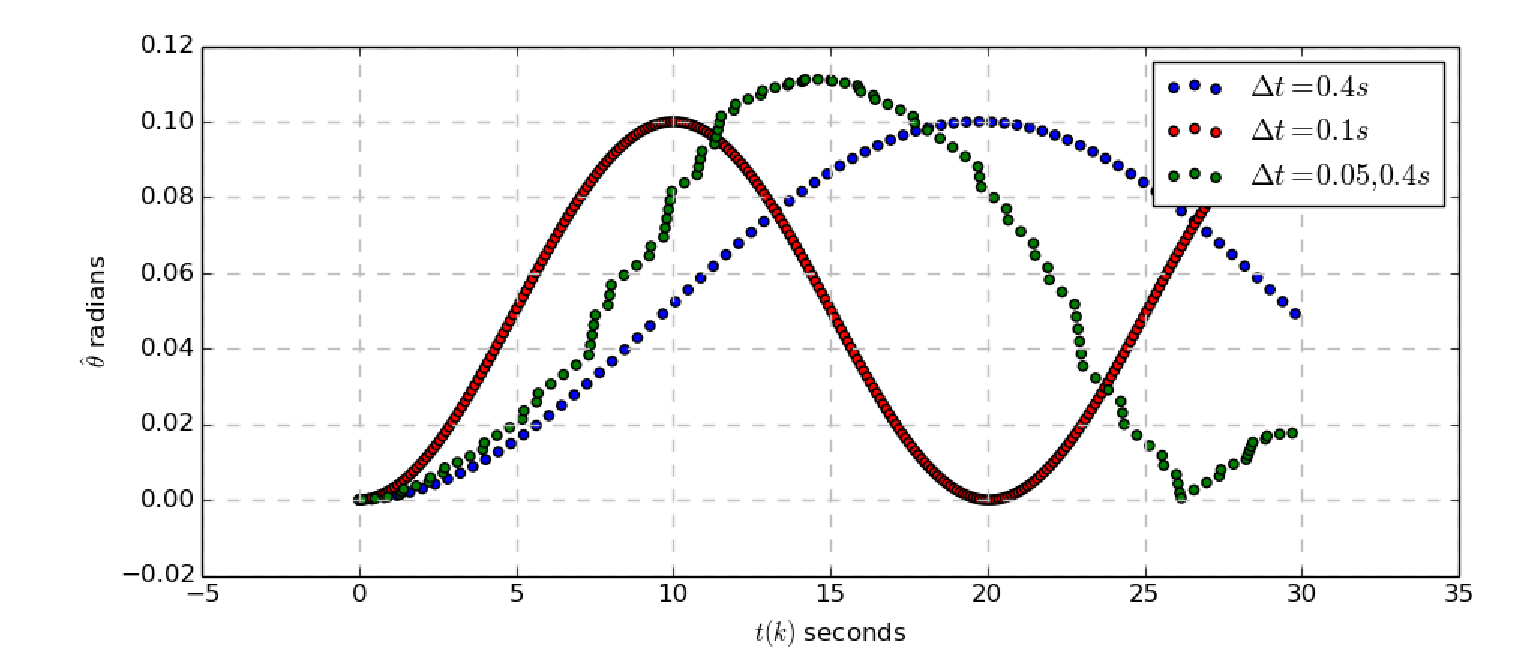
\psfig{file=figures/i_estimator_time_varying.eps,width=6in}}
  \caption{I-Estimator with time variation compensation}
  \label{fig:IEstimatorwithtimevariationcompensation}
\end{figure}

\subsection{Derivative State Estimation}
\label{subsec:DerivativeEstimator}

The derivative component of the PID estimator takes a similar form to the integral component in Equation \ref{eqn:IEstimator}.  The derivative component is only concerned with the current error, previous error, and the current time step size.  As with the integral body rate correction, the derivative correction is scaled by $\frac{1}{\Delta t_k}$ to compensate for variable step sizes.

\begin{subequations}
  \begin{align}
    \bs{\hat{x}}(t_{k+1}) &= \begin{bmatrix} \bs{\hat{q}}(t_{k+1}) \\ \bs{\hat{\omega}}(t_{k+1}) \end{bmatrix} \\
    \bs{\hat{q}}(t_{k+1}) &= \bs{\psi}\left(\bs{q}_{ed}(t_k), K_{qd}\right) \otimes \bs{\hat{q}}(t_{k}) \\
    \bs{q}_{ed}(t_k) &= \bs{\psi}\left(\bs{q}_e(t_{k-1})^* \otimes \bs{q}_e(t_{k}), \frac{1}{\Delta t_{k}}\right)\\
    \bs{\hat{\omega}}(t_{k+1}) &= \bs{\hat{\omega}}(t_{k}) + \bs{K}_{\omega d} \cdot \left(\frac{1}{\Delta t_k} \bs{I}\right) \cdot \bs{\omega}_e(t_{k})
  \end{align}
  \label{eqn:DEstimator}
\end{subequations}

The Figures \ref{fig:DEstimatorwithouttimevariationcompensation} and \ref{fig:DEstimatorwithtimevariationcompensation} below are the results of three test runs with the same set up update frequencies as with the integral component (0.1/sec, 0.4/sec, and varied).  For this comparison, the TableSat was simulated into a steady $0.01$ rad/s rotation about the body $+z$-axis to generate a constant rate of change for the quaternion instead of the fixed quaternion in the integral test.  The $\theta_{adj}$ parameter tracked for this test is the angular rotation associated with the $\bs{\psi}\left(\bs{q}_{ed}(t_k), K_{qd}\right)$ quaternion adjustment term.

\begin{figure}[H]
  \centerline{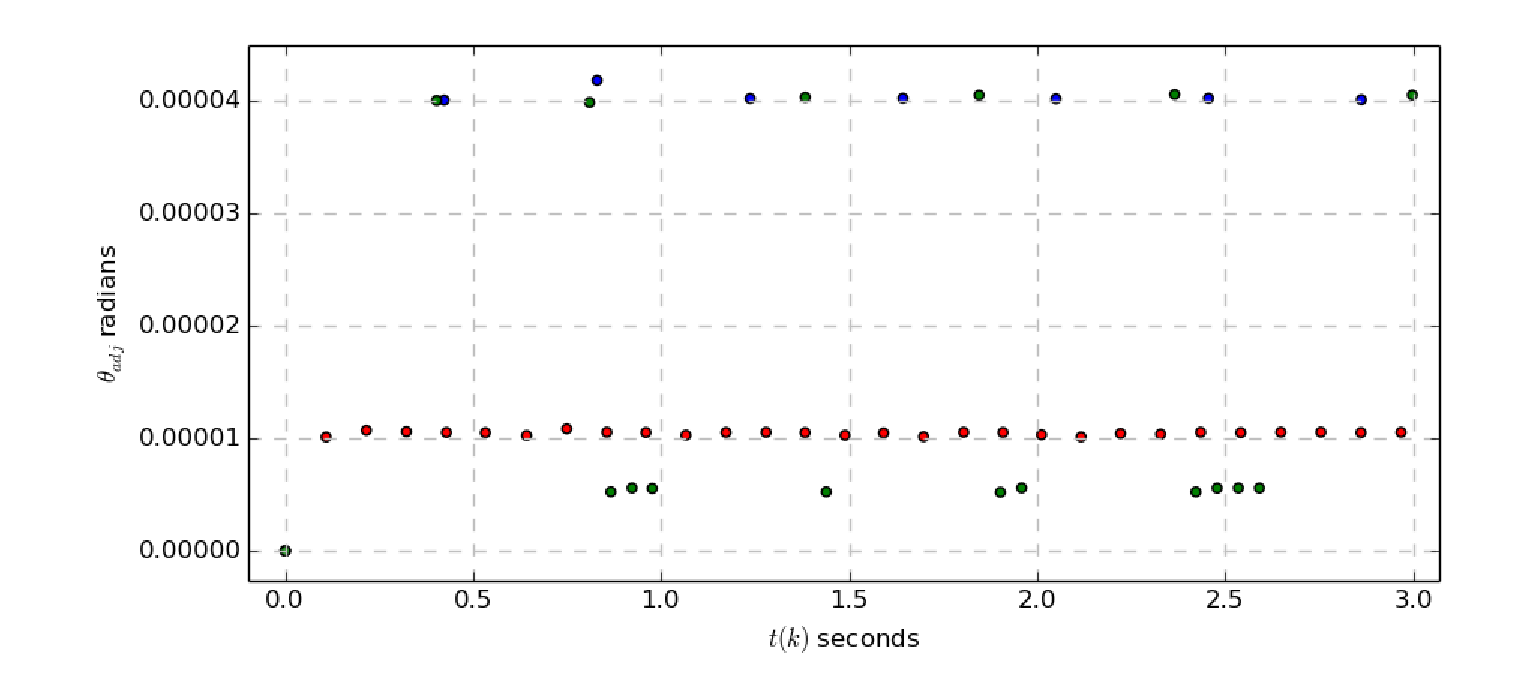
\psfig{file=figures/d_estimator_no_time_varying.eps,width=6in}}
  \caption{D-Estimator without time variation compensation}
  \label{fig:DEstimatorwithouttimevariationcompensation}
\end{figure}

Figure \ref{fig:DEstimatorwithouttimevariationcompensation} shows the results of the test run without consideration taken for time step sizes.  With a constant spin rate, the resulting quaternion adjustment is tightly coupled to the frequency that the updates are made with the 0.1 (red), 0.4 (blue), and variable 0.05/0.4 (green) time steps.  The variable time step sequence is a particular concerns as it jumps back and forth between adjusted amount suggesting the spin rate is not constant.

\begin{figure}[H]
  \centerline{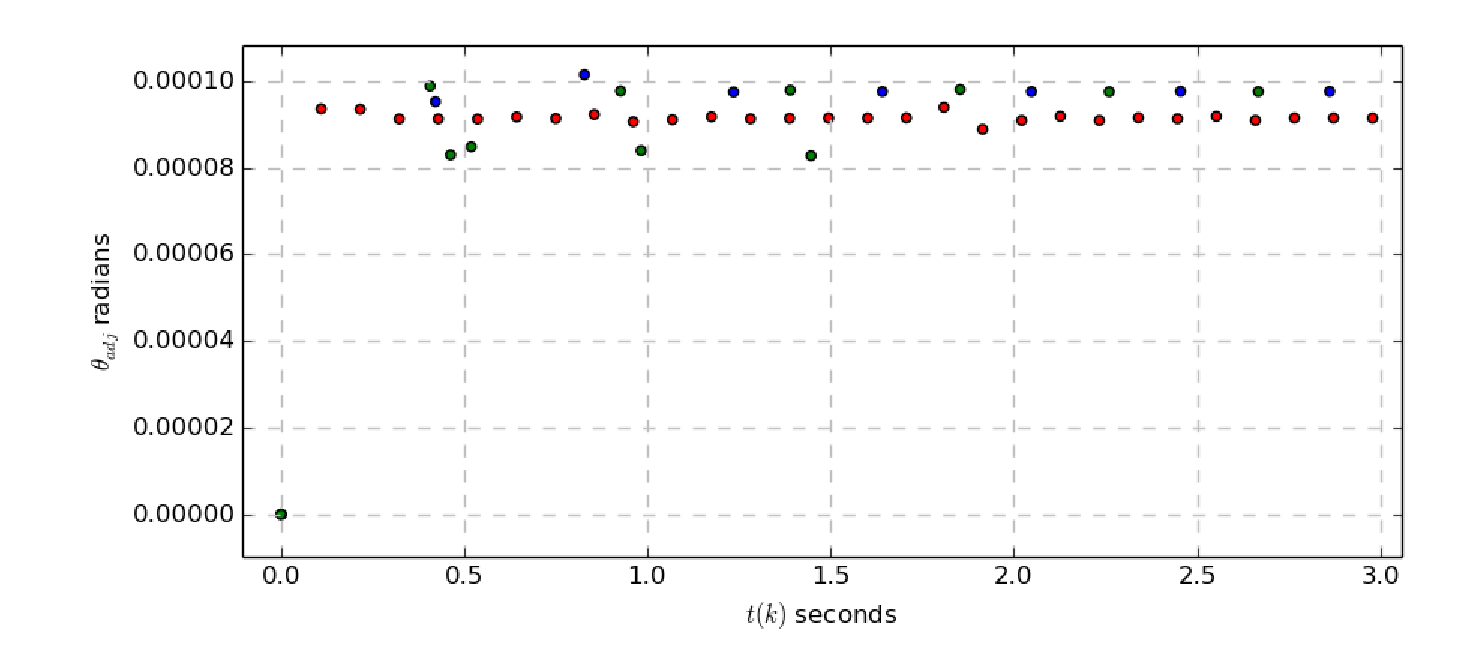
\psfig{file=figures/d_estimator_time_varying.eps,width=6in}}
  \caption{D-Estimator with time variation compensation}
  \label{fig:DEstimatorwithtimevariationcompensation}
\end{figure}

Figure \ref{fig:DEstimatorwithtimevariationcompensation} implements the time variation compensation in Equation \ref{eqn:DEstimator} where the quaternion adjustments provide a better representation of the measured constant spin rate.

\subsection{PID State Estimation of Unforced Motion}
\label{subsec:PIDEstimatorofUnforcedMotion}

Combining the proportional, integral, and derivative estimator portions from above.  Equations \ref{eqn:PEstimator}, \ref{eqn:IEstimator}, and \ref{eqn:DEstimator} get combined into a single PID estimator as

\begin{subequations}
  \begin{align}
    \bs{\hat{x}}(t_{k+1}) &= \begin{bmatrix} \bs{\hat{q}}(t_{k+1}) \\ \bs{\hat{\omega}}(t_{k+1}) \end{bmatrix} \\
    \bs{\hat{q}}(t_{k+1}) &= \bs{\psi}\left(\bs{q}_{ed}(t_k), K_{qd}\right) \otimes \bs{\psi}\big(\bs{q}_{ei}(t_k), K_{qi}\big) \otimes \bs{\psi}(\bs{q}_e(t_{k}), K_{qp})  \otimes \bs{\hat{q}}(t_{k}) \\
    \bs{\hat{\omega}}(t_{k+1}) &= \bs{\hat{\omega}}(t_{k}) + \bs{K}_{\omega p} \cdot \bs{\omega}_e(t_{k}) + \bs{K}_{\omega i} \cdot (\Delta t_k \bs{I})\cdot \bs{\omega}_e(t_{k}) + \bs{K}_{\omega d} \cdot \left(\frac{1}{\Delta t_k} \bs{I}\right) \cdot \bs{\omega}_e(t_{k})
  \end{align}
  \label{eqn:PIDEstimatorUnforcedMotion}
\end{subequations}

The update to the estimated body rate follows the traditional method of the PID control with the addition of the scaling factors for the integral and derivative terms that compensate for non-uniform step sizes at run-time.  The quaternion correction is a compilation of the individual correction quaternions and joined through the multiplicative error correction method.

With a spin-stabilized system controlling the body rate is relatively straight forward with a PID controller.  A test was run through TSatPy with based on the PID estimation in Equation \ref{eqn:PIDEstimatorUnforcedMotion}.  The system was set at a spin rate of $0.314$ rad/sec rotation about $+z$ with the measurement of the quaternion angle $\theta$ containing noise $N \sim (0, 0.1218)$ radians.  A gradient descent gain selection settled on the following parameters.

\begin{equation}
  \begin{aligned}
    K_{qp} &= 0.98, K_{qi} = 0.001, K_{qd} = 0.001 \\
    \bs{K}_{\omega p} &= 0.7 \bs{I}, \bs{K}_{\omega i} = \bs{0}, \bs{K}_{\omega d} = \bs{0}
  \end{aligned}
\end{equation}

The test run results are show in Figure \ref{fig:PIDEstimatorwithoutstateprediction}.  The bottom two graphs showing body rate tracking performance where the basic proportional control quickly brings the body rate error under control.  The quaternion estimations are much more difficult largely due to the lack of a system model to convert body rates to estimated attitudes at the next update.  Since the system is spin-stabilized and the estimated quaternion has no prior knowledge of where the next value will be, it relies on a large proportional component to jump to the new measurement values on each update.

While testing the performance of the integral and derivative components showed an improved performance when incorporating the effects of the variable time step, in this test with such a heavy reliance on the proportional component, the benefits to considering the variable time step effects were negligible.

\begin{figure}[H]
  \centerline{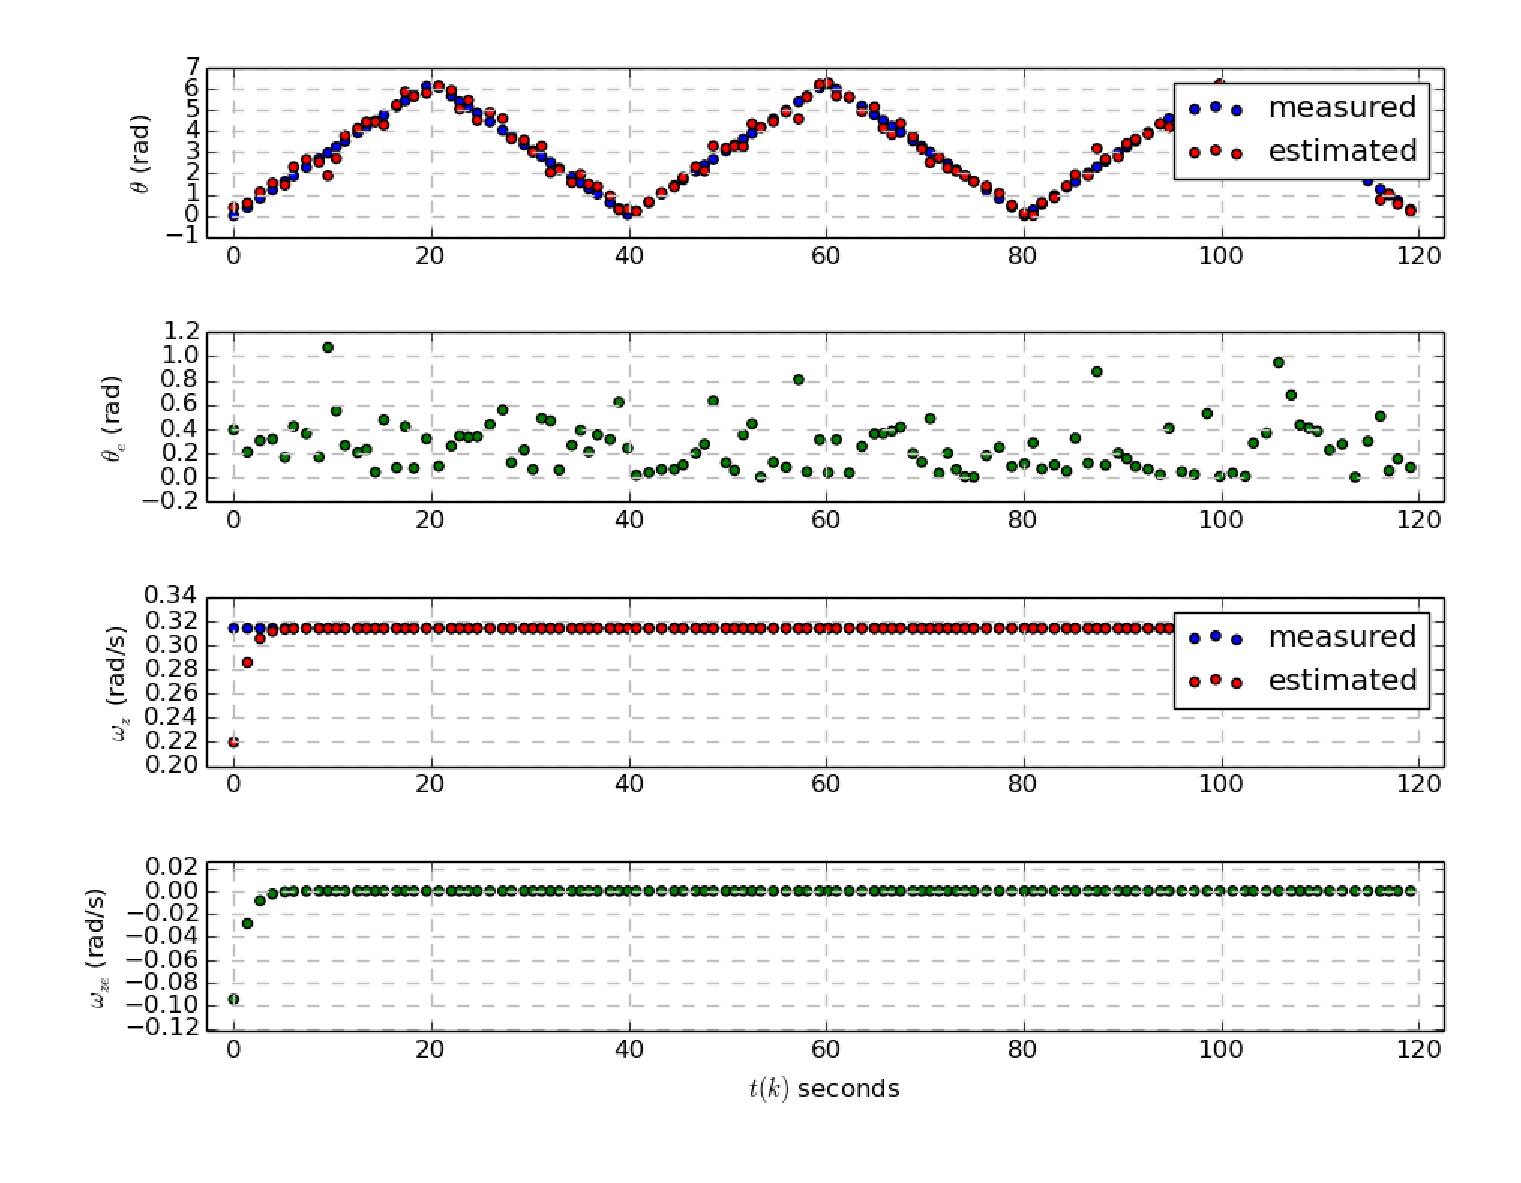
\psfig{file=figures/pid_estimator_no_prediction_high_P.eps,width=6in}}
  \caption{PID-Estimator without state prediction}
  \label{fig:PIDEstimatorwithoutstateprediction}
\end{figure}


\subsection{PID Estimation with State Prediction}
\label{subsec:PIDEstimatorwithStatePrediction}

From Section \ref{sec:BodyRatePIDEstimation}, Equation \ref{eqn:PIDEstimatorUnforcedMotion} defines a method of tracking unforced spin-stabilized satellites through PID state estimation.  The biggest issue was a heavy reliance on the proportional gain to track the quaternion attitude which is sensitive to measurement noise.  Incorporating a multiplicative-correction quaternion based model of rigid body dynamics based on the equations in Chapter \ref{chap:SatelliteAttitudeModeling} can assist in predicting the $t_{k+1}$ state of the system.

\begin{subequations}
  \begin{align}
    \bs{\hat{x}}(t_{k+1}) &= \begin{bmatrix} \bs{\hat{q}}(t_{k+1}) \\ \bs{\hat{\omega}}(t_{k+1}) \end{bmatrix} \\
    \bs{\hat{q}}(t_{k+1}) &= \bs{\psi}\left(\bs{q}_{ed}(t_k), K_{qd}\right) \otimes \bs{\psi}\big(\bs{q}_{ei}(t_k), K_{qi}\big) \otimes \bs{\psi}(\bs{q}_e(t_{k}), K_{qp})  \otimes \bs{\hat{q}}(t_{k+1})^- \\
    \bs{\hat{\omega}}(t_{k+1}) &= \bs{\hat{\omega}}(t_{k+1})^- + \bs{K}_{\omega p} \cdot \bs{\omega}_e(t_{k}) + \bs{K}_{\omega i} \cdot (\Delta t_k \bs{I})\cdot \bs{\omega}_e(t_{k}) + \bs{K}_{\omega d} \cdot \left(\frac{1}{\Delta t_k} \bs{I}\right) \cdot \bs{\omega}_e(t_{k})
  \end{align}
  \label{eqn:PIDEstimatorwithPredictionUnforcedMotion}
\end{subequations}

with the a priori state $\bs{\hat{x}}(t_{k+1})^-$ as

\begin{equation}
  \bs{\hat{x}}(t_{k+1})^- = \begin{bmatrix}\bs{\hat{q}}(t_{k+1})^- \\ \bs{\hat{\omega}}(t_{k+1})^- \end{bmatrix} = f \Big( \bs{\hat{q}}(t_{k}), \bs{\hat{\omega}}(t_{k}) \Big)
\end{equation}

The PID estimator now with a state prediction method was run under the same testing conditions present in Figure \ref{fig:PIDEstimatorwithoutstateprediction}.  The resulting performance showed that the inclusion of the system model greatly reduced the reliance on the proportional component of the PID estimator which reduced the noise and increased the accuracy of the final estimates being provided to the controller.  The results in Figure \ref{fig:PIDEstimatorwithstateprediction} show the improved quaternion angle estimates when run with the following gains.

\begin{equation}
  \begin{aligned}
    K_{qp} &= 0.0735, K_{qi} = 0.000863, K_{qd} = 0.00812 \\
    \bs{K}_{\omega p} &= 0.7 \bs{I}, \bs{K}_{\omega i} = \bs{0}, \bs{K}_{\omega d} = \bs{0}
  \end{aligned}
\end{equation}

The quaternion's proportional value is still the dominant gain, but has been reduced by 92.5\% of it's previous value while still providing about 80\% reduction in quaternion attitude error rates.

\begin{figure}[H]
  \centerline{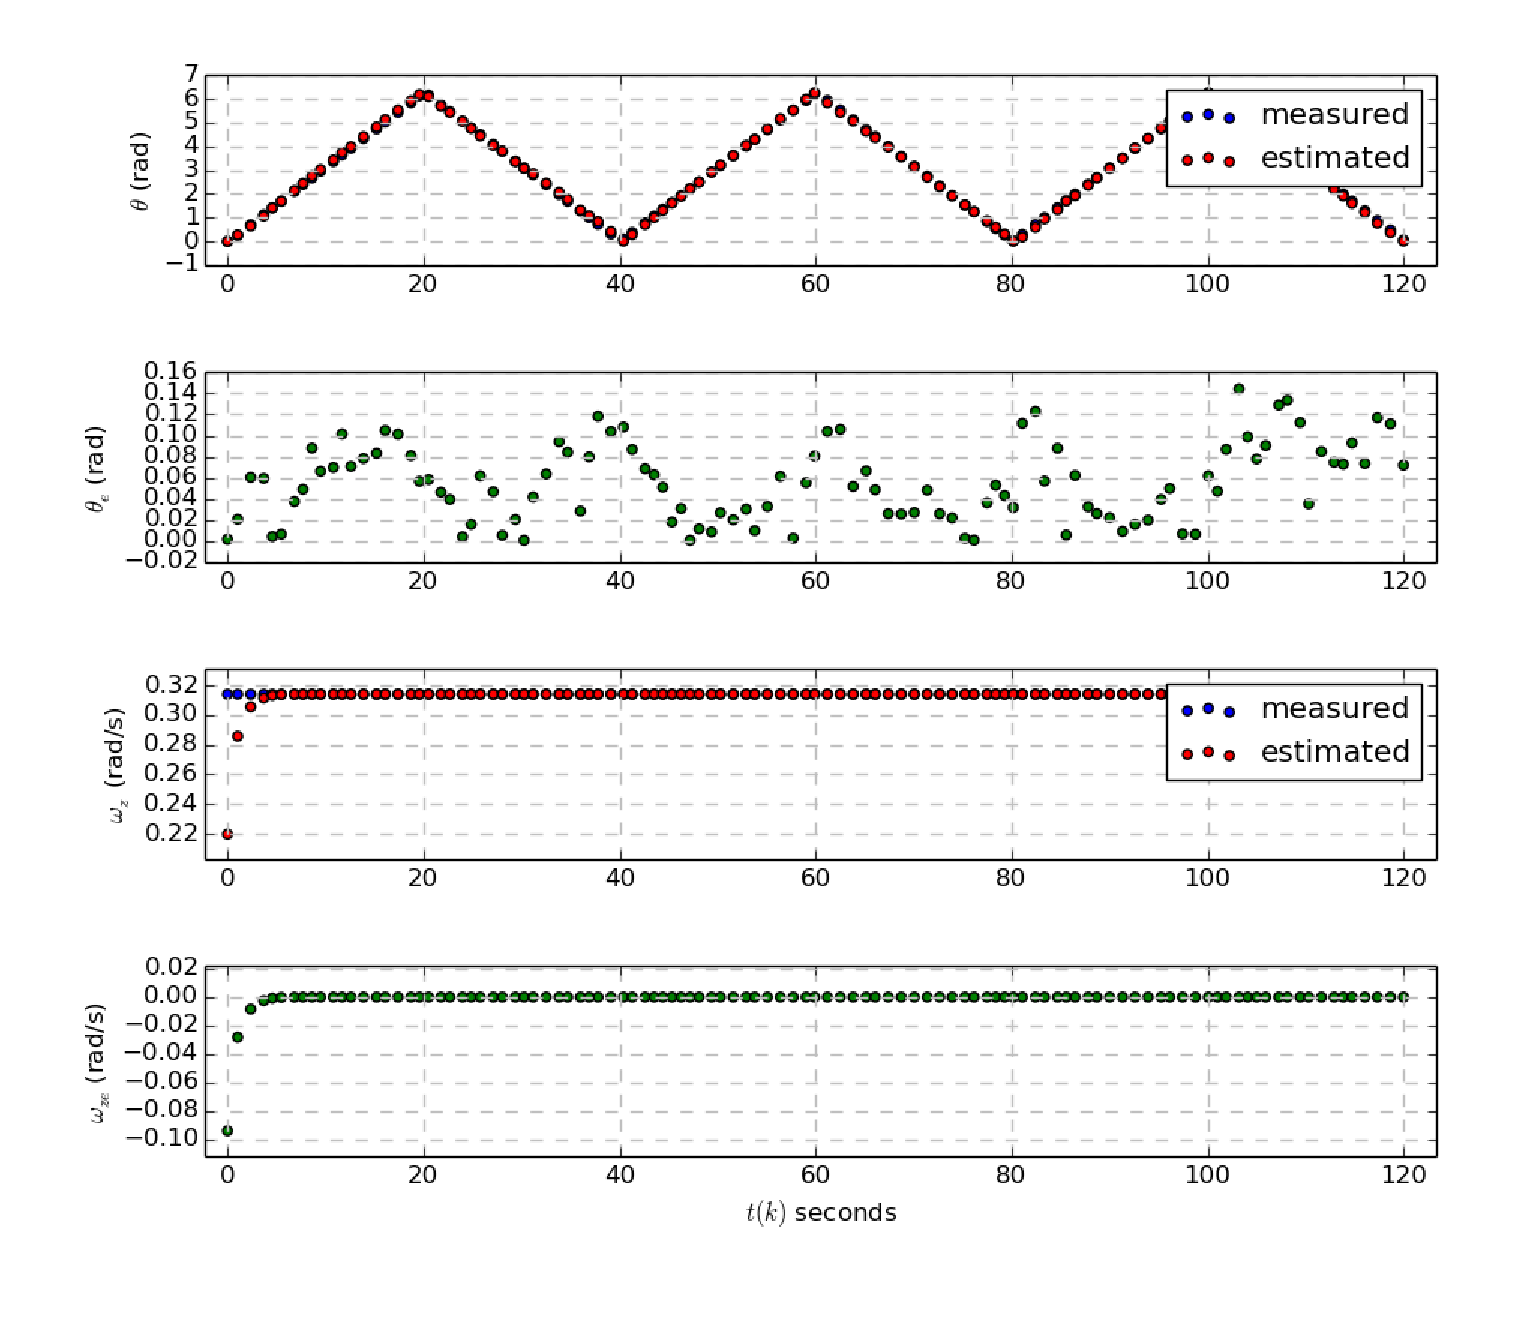
\psfig{file=figures/pid_estimator_with_prediction.eps,width=6in}}
  \caption{PID-Estimator with state prediction}
  \label{fig:PIDEstimatorwithstateprediction}
\end{figure}


\section{Sliding Mode Observer with State Prediction}
\label{sec:SlidingModeObserverwithStatePrediction}

The Sliding Mode Observer (SMO) is a proportional estimator with an additional smoothing term that uses a chosen sliding surface.  The general form for the SMO is

\begin{equation}
  \bs{\dot{\hat{x}}} = \bs{\hat{f}}(\bs{\hat{x}}, \bs{\hat{u}}, t) + \bs{L}(\bs{C}\bs{\hat{x}} - \bs{C}\bs{x}) + \bs{K}\bs{1}_s\bs{\hat{y}}
  \label{eqn:SMOContinuous}
\end{equation}

Where L is a luenberger gain and $\bs{1}_s$ is a switching function based on $s$.  The sliding mode terms allow additional control of the state adjustments without adding a lot of computational complexity.  The SMO can continue to use the nonlinear model's state predictions as in the PID estimators in Section \ref{subsec:PIDEstimatorwithStatePrediction}, which is an advantage over methods such as the Extended Kalman Filter (EKF) where the system is linearized about an operating point and assumes a constant time step.

This thesis takes the discretized form of Equation \ref{eqn:SMOContinuous} with a quaternion multiplicative correction

\begin{subequations}
  \begin{align}
    \bs{\hat{x}}(t_{k+1}) &= \begin{bmatrix} \bs{\hat{q}}(t_{k+1}) \\ \bs{\hat{\omega}}(t_{k+1}) \end{bmatrix} \\
    \bs{\hat{q}}(t_{k+1}) &= \bs{\psi} (\bs{1}_s\big(\bs{q}_{e}(t_k)\big), K_q) \otimes \bs{\psi}(\bs{q}_e(t_{k}), L_{q})  \otimes \bs{\hat{q}}(t_{k+1})^- \\
    \bs{\hat{\omega}}(t_{k+1}) &= \bs{\hat{\omega}}(t_{k+1})^- + \bs{L}_{\omega} \bs{\omega}_e(t_{k}) + \bs{K}_{\omega}\bs{1}_s \big(\bs{\omega}_e(t_{k}) \big)
  \end{align}
  \label{eqn:SMOEstimatorwithPredictionUnforcedMotion}
\end{subequations}

where

\begin{subequations}
  \begin{align}
    \bs{1}_s\big(\bs{q}_{e}(t_k) \big) &= \begin{bmatrix} \bs{v_e} \\ sat\left( \frac{2\cos^{-1} q_{0e} }{S_{q}} \right) \end{bmatrix} \\
    \bs{1}_s \big(\bs{\omega}_e(t_{k}) \big) &= sat\left( \frac{\bs{\omega}_e(t_{k})}{S_{\omega}} \right) \\
    \bs{L}_{\omega} &= L_\omega \cdot \bs{I} \\
    \bs{K}_{\omega} &= K_\omega \cdot \bs{I}
  \end{align}
\end{subequations}

For body rates, the a priori state provides the predicted body rate $\bs{\hat{\omega}}(t_{k+1})^-$ that gets adjusted by a proportional term $\bs{L}_{\omega} \bs{\omega}_e(t_{k})$ as in the P-Estimator, but has an additional saturation function correction based on sliding surfaces for the individual body rate errors.  As found in the PID estimator, the proportional estimator for a steady spin-stabilized satellite performs adequately.  The additional saturation term becomes helpful for situations with low $L_\omega$ values that can take longer to converge from the initial body rate to the actual body rate, but once close will increase the effort in staying in step with the measured body rate.

Similar to the PID estimator, the quaternion sliding mode observer limits it's focus to the angular measure of the rotational quaternion.  The sliding surface is taken based on the radian measure.  If the radian measure is below, the saturation limit the quaternion stays as is.  If the quaternion represents a rotation greater than the saturation limit a saturated quaternion is created about the same Euler axis but limit to the saturation angle of rotation.

Running the same tests as run against the PID estimators, the following parameters were located through an iterative gradient descent method that minimized the quaternion error angle and standard deviation of the error angle.

\begin{equation}
  \begin{aligned}
    L_q = 0.362 &, L_w = 0.375 \\
    K_q = 0.308 &, K_w = 0.499 \\
    S_q = 0.419 &, S_w = 0.00517 \\
  \end{aligned}
\end{equation}

Figure \ref{fig:SMOEstimatorwithstateprediction} shows the result of the test at these optimized parameters.  The inverted angle measurement in the first graph is an artifact of the non-unique representation of a quaternion attitude.  In this case, the estimated angles are being calculated for rotations about the body's $-z$-axis instead of the $+z$ axis.  This further supports the decision made in Section \ref{chap:StateError} to use the multiplicative error as the second graph shows the correct error values.

Although the SMO in this case is able to traverse the initial transient response well, the steady state quaternion error is almost as high as using a PID estimator with no state prediction method.  This behavior is due to the high quaternion measurement noise.  With the saturation function, the sliding mode observer is still largely a proportional estimator without the assistance of an integral term to smooth out the noise.

\begin{figure}[H]
  \centerline{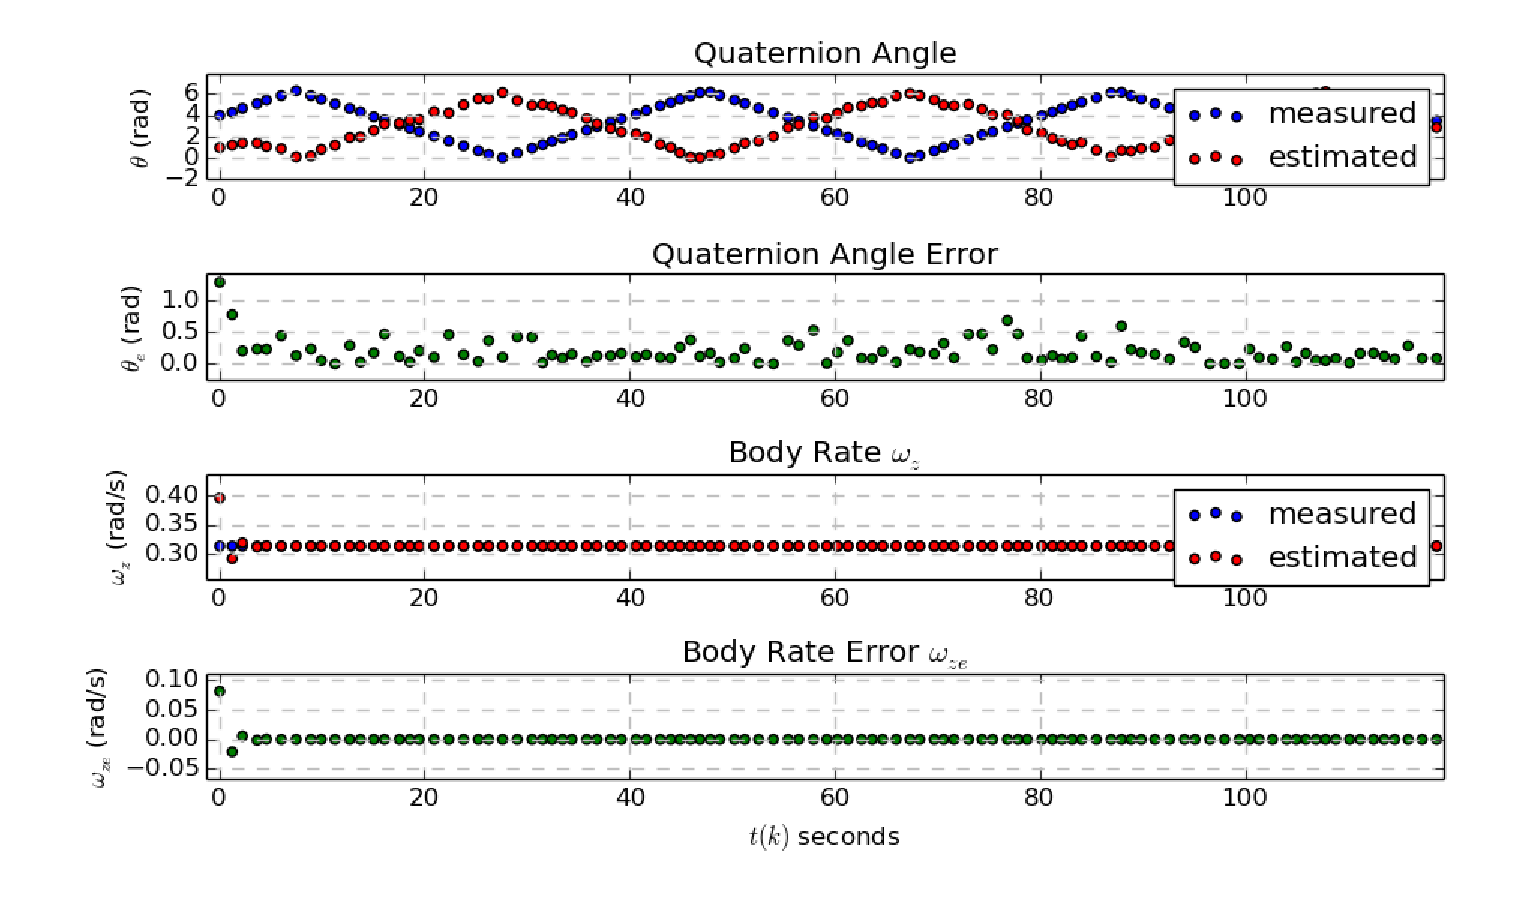
\psfig{file=figures/smo_estimator_with_prediction.eps,width=6in}}
  \caption{SMO-Estimator with state prediction}
  \label{fig:SMOEstimatorwithstateprediction}
\end{figure}

Based on these results, the SMO performs acceptably for the body rate estimation, but according to the steady state error rates, it appears that the PID estimation would be a better use for the steady state attitude tracking.  Both estimators have similar performance profiles which makes it more complicated to determine the better choice.  Section \ref{sec:ComparativeAnalysysofPIDandSMOEstimators} will go over how TSatPy can assist with running both estimation techniques in parallel for to provide a more accurate representation.

\section{Comparative Analysis of PID and SMO Estimators}
\label{sec:ComparativeAnalysysofPIDandSMOEstimators}

One of the advantages to developing the TSatPy code base for the MMS/TableSat spin-stabilized is the ability to run a comparative analysis of multiple estimators at the same time.  The estimators run agnostic to the source of the measurements.  In the sample shown below, the state measurements were generated by a model, but could also be switched to be pulled off the TableSat.

Figure \ref{fig:PIDSMOEstimatorConcurrentComparison} was generated by running a single simulation an providing the truth model's measured state to both a PID and SMO estimator tuned to the parameters selected during individual gain tuning tests above.  This allows for a clear side-by-side comparison of their performance.  Multiple runs all have similar characteristics.  In the initial transient response both estimators are able to converge to a steady state after just a couple updates, but the SMO is able to converge slightly faster each time.  For the steady state response the PID estimator consistently maintains a lower average error, although with a slightly higher standard deviation.  As with the initial response, the SMO estimation values generally update slightly just before the PID estimator.

\begin{figure}[H]
  \centerline{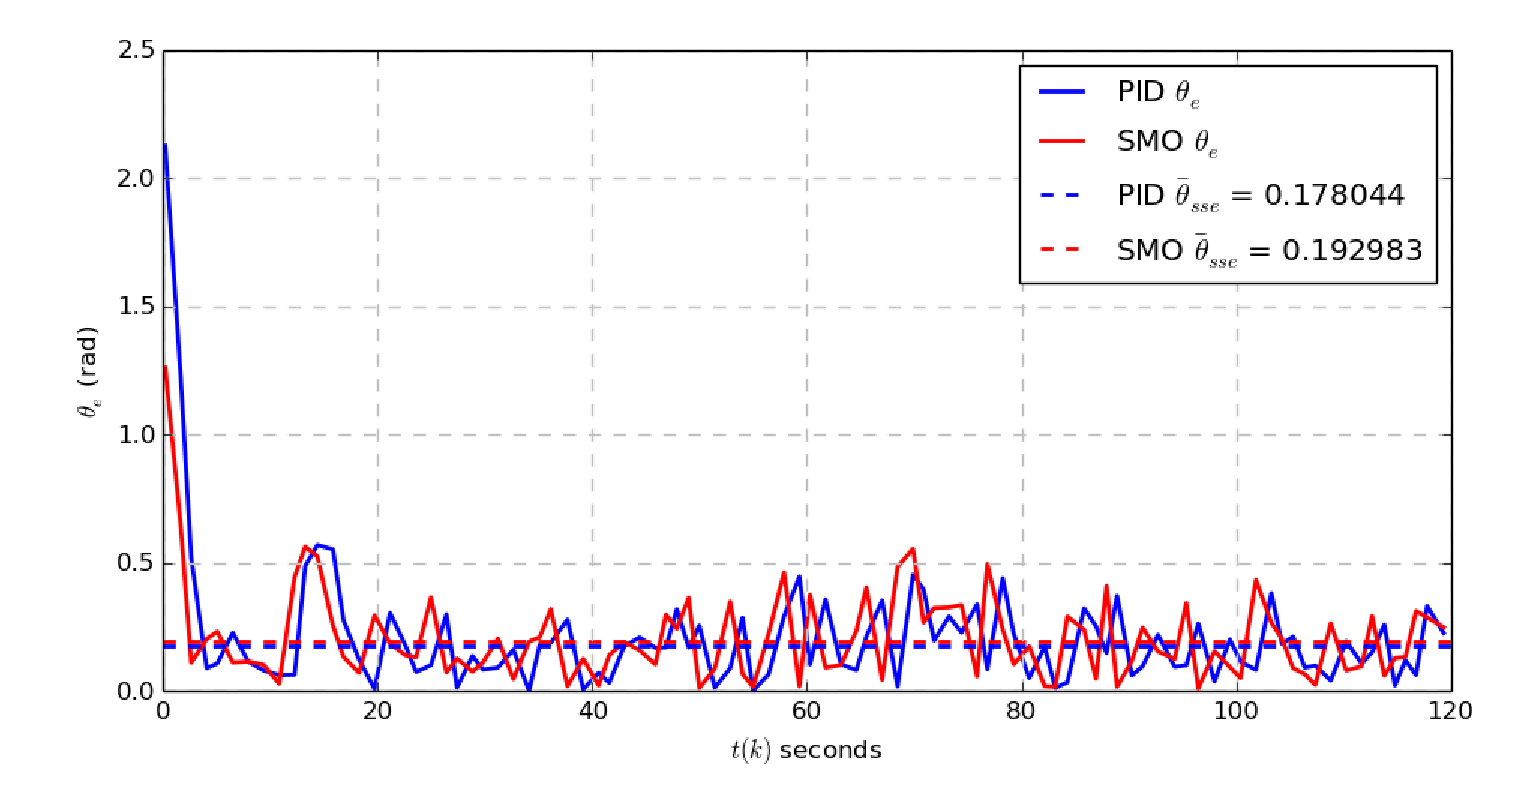
\psfig{file=figures/estimator_comparison.eps,width=6in}}
  \caption{PID/SMO Estimator Concurrent Comparison}
  \label{fig:PIDSMOEstimatorConcurrentComparison}
\end{figure}

The results in Figure \ref{fig:PIDSMOEstimatorConcurrentComparison} were generated through the TSatPy application with the script below.  Lines 10-15 define the two estimators to use in the simulation.  More can be added including the same estimator type with varied parameters.  Lines 17-19 define the system clock behavior.  The simulation will run for a simulated 120 seconds as verified in the results above.  The time steps for each update will vary between 0.8 and 1.2 seconds randomly.  And since this is running as a simulation instead of pulling data from the physical TableSat, the clock can be sped up to run at 10x speed improving the rate of the iterative testing cycle.

\begin{singlespace}
  \begin{minted}[mathescape,linenos,numbersep=10pt,frame=lines,framesep=2mm]{python}
from TSatPy import Estimator, State
from TSatPy.Clock import Metronome
import numpy as np
import matplotlib.pyplot as plt
import time
import random

print('PID / SMO Faceoff')

configs = [{'type': 'pid',
 'args': {'kpq': 0.0735,'kpw': 0.7,'kiq': 0.000863,
          'kiw': 0,'kdq': 0.00812,'kdw': 0}
},{'type': 'smo',
 'args': {'Lq': 0.3619,'Lw': 0.3752,'Kq': 0.3076,
           'Kw': 0.4994,'Sq': 0.4191,'Sw': 0.0052}}]

run_time = 120
speed = 10
dts = [0.8, 1.2]
c = Metronome()
c.set_speed(speed)
I = [[2, 0,  0], [0, 2, 0], [0, 0, 2]]

def setup_estimators(configs):
    x_ic = State.State()
    plant_est = State.Plant(I, x_ic, c)

    est = Estimator.Estimator(c)
    for config in configs:
        est.add(config['type'], plant_est, config['args'])

    return est

def run_comparison(est):
    x_ic = State.State(
        State.Quaternion([0,0,1], radians=4),
        State.BodyRate([0,0,0.314]))
    plant = State.Plant(I, x_ic, c)

    ts = []; smo_err = []; pid_err = []
    start_time = c.tick()
    end_time = c.tick() + run_time
    while c.tick() < end_time:
        plant.propagate()
        offset = np.random.randn() * 20 / 180.0 * np.pi
        q_noise = State.Quaternion([0,0,1], radians=offset) * plant.x.q

        x_m = State.State(q_noise, plant.x.w)

        est.update(x_m)
        ts.append(c.tick() - start_time)

        for model in est.estimators:
            q_e = State.QuaternionError(model.x_hat.q, plant.x.q)
            e, r = q_e.to_rotation()

            if type(model) is Estimator.PID:
                pid_err.append(r)
            elif type(model) is Estimator.SMO:
                smo_err.append(r)
        random.shuffle(dts)
        time.sleep(dts[0] / float(speed))

    return ts, pid_err, smo_err

def graph_it(ts, pid_err, smo_err):
    # Generate the graph here
    # See appendix for the full script

def main():
    est = setup_estimators(configs)
    graph_it(*run_comparison(est))
    return 0

if __name__ == '__main__':
    exit(main())
  \end{minted}
\nocite{minted}
\end{singlespace}

The TableSat 1A controller has performance requirements based off of NASA MMS's mission parameters.  Section \ref{sec:ComparativeAnalysysofPIDandSMOEstimators} demonstrated that multiple estimators can be run in parallel during both simulations and experimental runs.  As discussed above, this allows for a better insight into performance differences in estimation methods.  An additional benefit to running the controller through TSatPy is the ability to perform estimator scheduling.  Like gain scheduling which for an estimator or controller can modify what gains it uses depending on the current performance, estimator scheduling allows for switching between disparate estimation techniques during run-time.  For example, one estimator tuned for responding to large errors and run along side an estimator tuned for steady state performance.  The control algorithm can then receive more accurate state estimates on a wider range of environmental conditions.
